\documentclass[aspectratio=169]{beamer}
\usepackage[utf8]{inputenc}
\usepackage[T1]{fontenc}
\usepackage{booktabs}
\usepackage{colortbl}
\usepackage{graphicx}
\usepackage{xcolor}
\usepackage{tikz}
\usetikzlibrary{positioning}
\usepackage{pgfplots}
\pgfplotsset{compat=1.18}
\usepackage{amsmath}
\usepackage{tcolorbox}
\tcbuselibrary{skins}

\definecolor{cdark}{HTML}{0D2137}
\definecolor{cmid}{HTML}{065A82}
\definecolor{cteal}{HTML}{02C39A}
\definecolor{clight}{HTML}{E8F4F8}
\definecolor{ctext}{HTML}{1A2E40}
\definecolor{cmuted}{HTML}{607D8B}
\definecolor{cwarn}{HTML}{F4A261}
\definecolor{cgap}{HTML}{E63946}
\definecolor{caccent}{HTML}{A0BFD0}
\definecolor{cbg2}{HTML}{028090}

\usetheme{default}
\usecolortheme{default}
\setbeamertemplate{navigation symbols}{}
\usefonttheme{professionalfonts}
\setbeamerfont{frametitle}{size=\large,series=\bfseries}
\setbeamercolor{frametitle}{fg=cdark,bg=white}
\setbeamercolor{normal text}{fg=ctext}
\setbeamercolor{background canvas}{bg=white}
\setbeamercolor{item}{fg=cteal}

\addtobeamertemplate{frametitle}{}{%
  \vspace{-4pt}\textcolor{cteal}{\hrule height 1.5pt}\vspace{3pt}}

\setbeamertemplate{footline}{%
  \leavevmode\hbox{%
    \begin{beamercolorbox}[wd=0.85\paperwidth,ht=2.2ex,dp=1ex,leftskip=4pt]{normal text}%
      \tiny\color{cmuted}An Pham \textbar{} LIRMM--ADVANSE \textbar{} Luc \& Reda%
    \end{beamercolorbox}%
    \begin{beamercolorbox}[wd=0.15\paperwidth,ht=2.2ex,dp=1ex,right,rightskip=6pt]{normal text}%
      \scriptsize\color{cmuted}\insertframenumber/\inserttotalframenumber%
    \end{beamercolorbox}}}

\setbeamertemplate{itemize item}{\color{cteal}\textbullet}
\setbeamertemplate{itemize subitem}{\color{cmid}--}
\setlength{\leftmargini}{1em}

\newcommand{\statcard}[3]{%
  \begin{tcolorbox}[enhanced,boxrule=1pt,arc=2pt,
      colback=clight,colframe=cmid,
      top=3pt,bottom=3pt,left=3pt,right=3pt]
    \centering
    {\color{cmid}\large\bfseries\parbox[c][2.7em][c]{\linewidth}{\centering #1}}\\[1pt]
    {\color{ctext}\bfseries\tiny\parbox[c][2.8em][c]{\linewidth}{\centering #2}}\\[1pt]
    {\color{cmuted}\tiny\parbox[c][2.8em][c]{\linewidth}{\centering #3}}
  \end{tcolorbox}}

\title{\textbf{PICOPATT Internship}}
\subtitle{Quick Progress Update --- May 2026}
\author{An Pham}
\institute{LIRMM--ADVANSE, Universit\'e de Montpellier}
\date{May 7, 2026}

\begin{document}

% ── SLIDE 1 ──────────────────────────────────────────────────────────────────
{\setbeamercolor{background canvas}{bg=cdark}
\begin{frame}[plain]
\begin{tikzpicture}[remember picture,overlay]
  \fill[cteal](current page.north west)rectangle([xshift=6pt]current page.south west);
\end{tikzpicture}
\vspace{1.1cm}
{\color{white}\huge\bfseries PICOPATT Internship}\\[5pt]
{\color{cteal}\large\itshape Quick Progress Update --- May 2026}\\[8pt]
{\color{caccent}\small Explainable Clustering for Spatio-Temporal Picoclimatic Data}\\[0.6cm]
{\color{cmid}\rule{4.5cm}{0.8pt}}\\[5pt]
{\color{caccent}\footnotesize\textbf{An Pham}\quad|\quad LIRMM--ADVANSE\quad|\quad Supervisors: Luc \& Reda}\\[2pt]
{\color{caccent}\footnotesize May 7, 2026}
\end{frame}}

% ── SLIDE 2 ──────────────────────────────────────────────────────────────────
\begin{frame}{Snapshot}
\begin{columns}[T,onlytextwidth]
  \column{0.25\textwidth}
  \statcard{4}{Proxy datasets}{ECG200, ECG5000, Synth. pico, Roma}
  \column{0.25\textwidth}
  \statcard{6}{Seeds for stability}{Feature overlap + fidelity}
  \column{0.25\textwidth}
  \statcard{5 OK}{Research scripts (Apr 27)}{0 failed; outputs archived}
  \column{0.25\textwidth}
  \statcard{8 figs}{Exported visuals}{Slides + SHAP/LIME assets}
\end{columns}
\vspace{0.25cm}
\begin{itemize}\footnotesize\setlength\itemsep{2pt}
  \item All numbers/figures sourced from archived runs under \texttt{outputs/}.
\end{itemize}
\end{frame}

% ── SLIDE 3 ──────────────────────────────────────────────────────────────────
\begin{frame}{Cross-dataset summary}
\centering
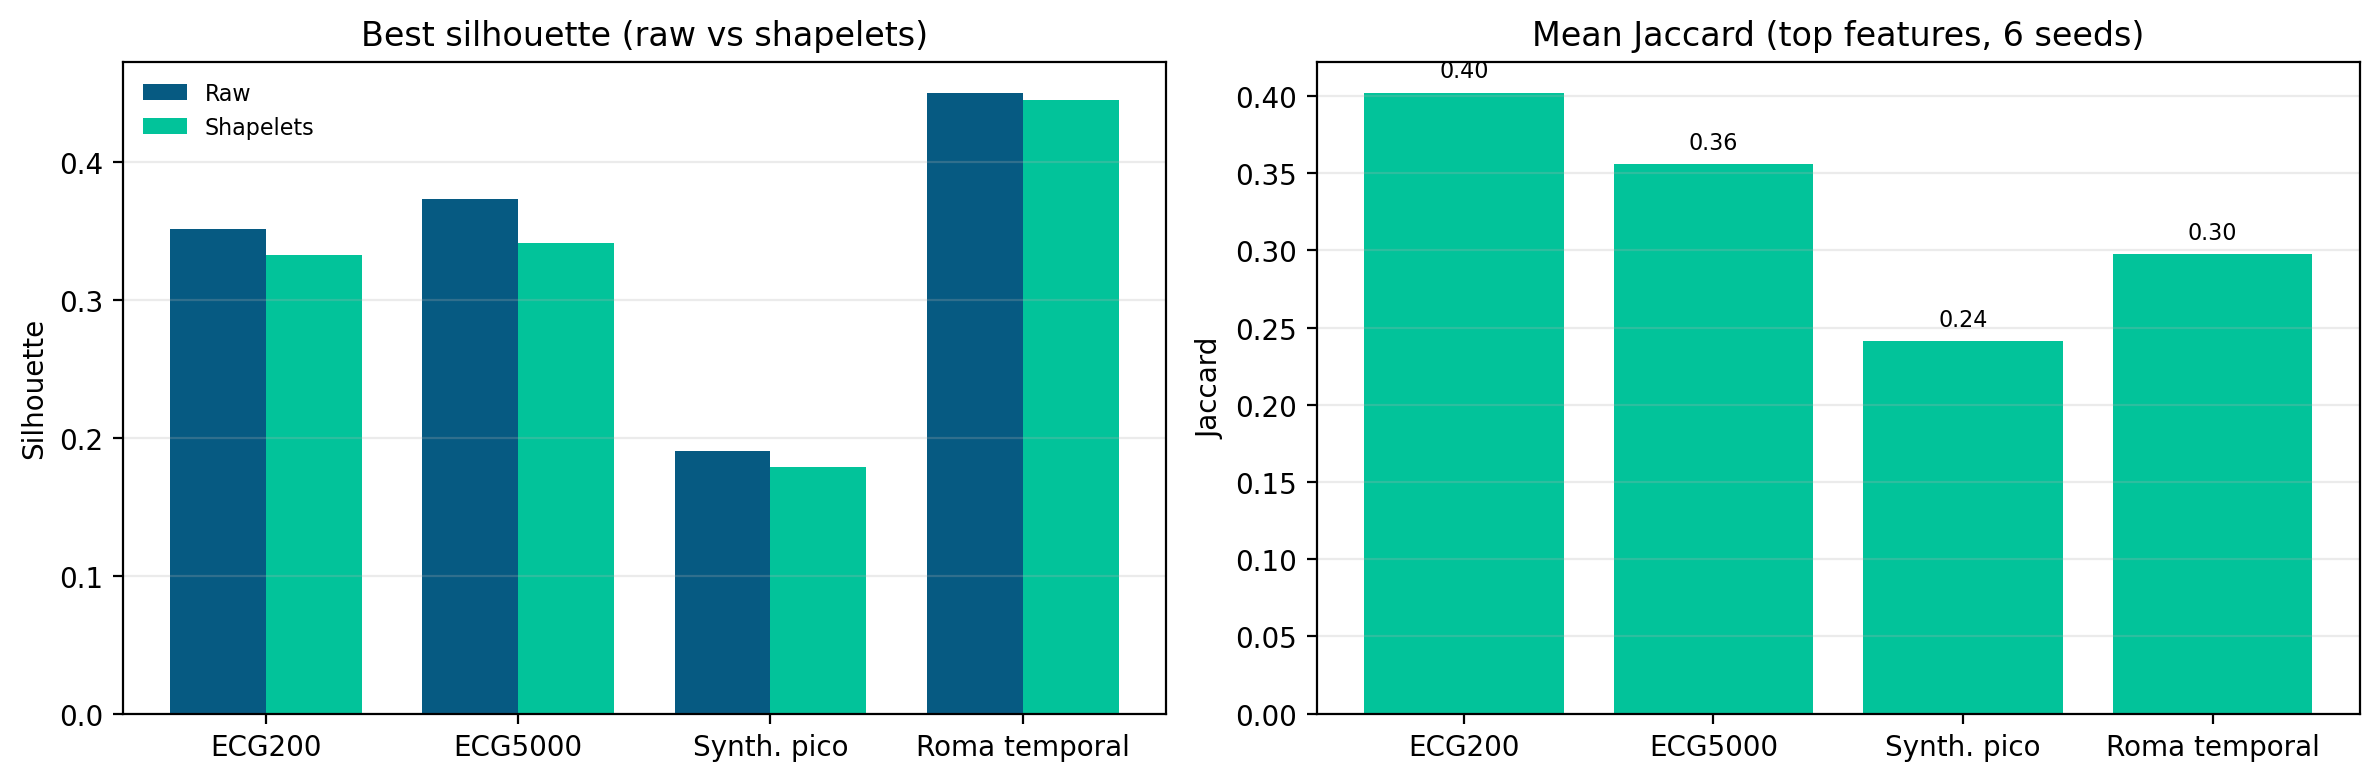
\includegraphics[width=0.92\linewidth,height=0.70\textheight,keepaspectratio]{figures/cross_dataset_summary.png}
\end{frame}

% ── SLIDE 4 ──────────────────────────────────────────────────────────────────
\begin{frame}{Stability evidence (6 seeds)}
\centering
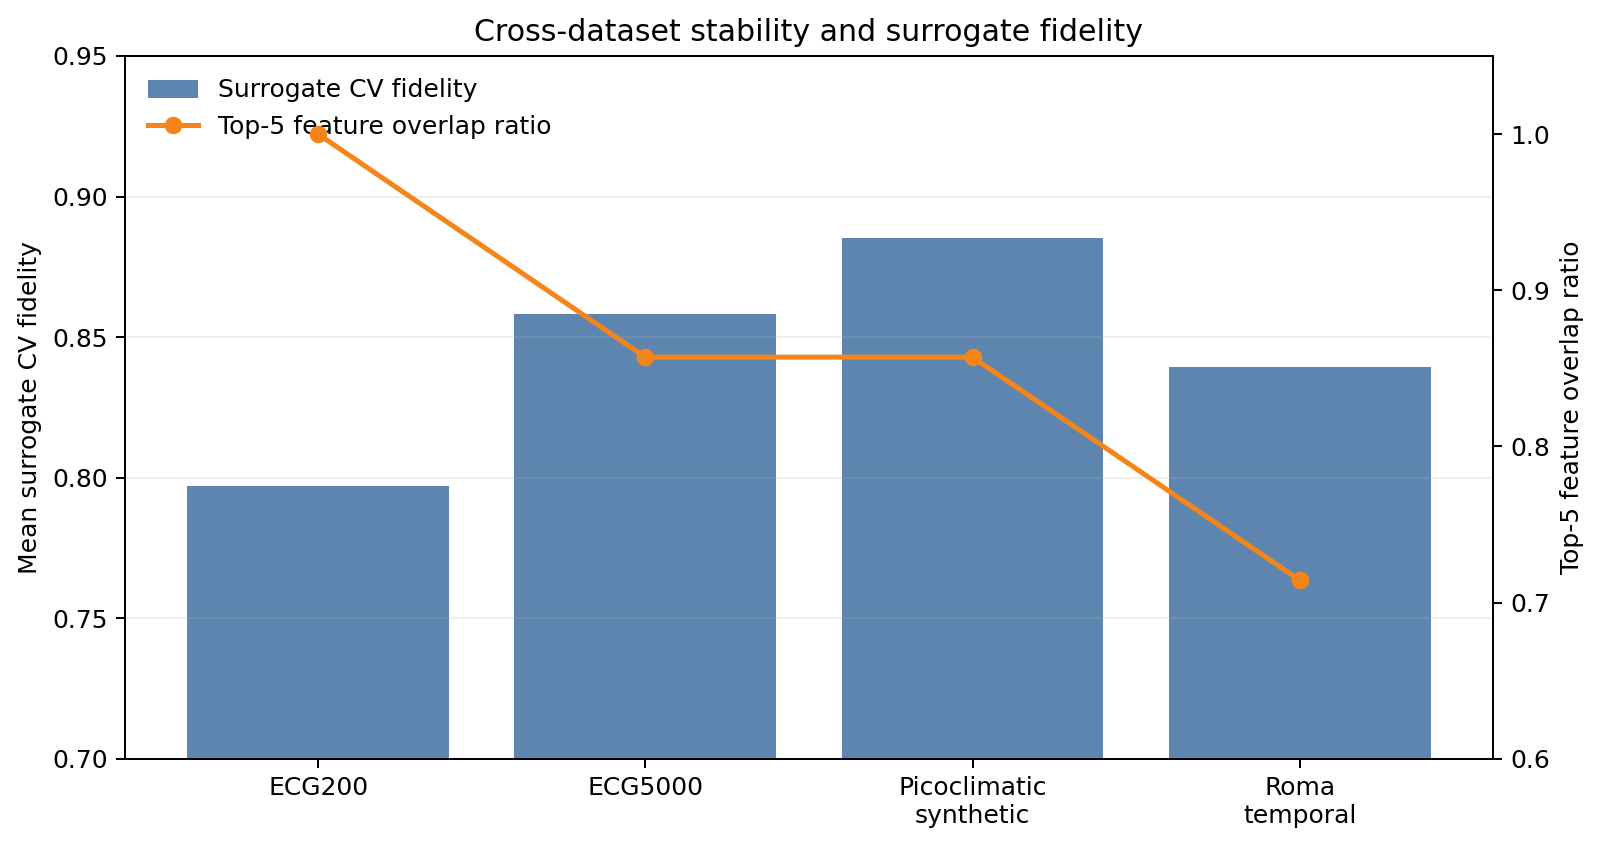
\includegraphics[width=0.96\linewidth,height=0.75\textheight,keepaspectratio]{figures/stability_summary.png}
\end{frame}

% ── SLIDE 5 ──────────────────────────────────────────────────────────────────
\begin{frame}{Explanation pipeline outputs (global)}
\begin{columns}[T,onlytextwidth]
  \column{0.52\textwidth}
  \centering
  \resizebox{0.98\linewidth}{!}{%
  \begin{tikzpicture}[
      pipelinebox/.style={
        draw=cmid,
        rounded corners=2pt,
        fill=white,
        align=center,
        inner xsep=4pt,
        inner ysep=3pt,
        minimum height=2.6em,
        text width=1.55cm,
        font=\scriptsize,
      },
      pipelinearrow/.style={->,>=Stealth,thick,draw=cmid},
      node distance=2.2mm,
    ]
    \node[pipelinebox] (a) {Window\\features\\{\tiny (142 vars)}};
    \node[pipelinebox, right=of a] (b) {K-Means\\pseudo-labels};
    \node[pipelinebox, right=of b] (c) {Surrogate\\RF\\classifier};
    \node[pipelinebox, right=of c] (d) {SHAP\\global\\importance};
    \node[pipelinebox, right=of d] (e) {LIME\\local\\rationale};

    \draw[pipelinearrow] (a.east) -- (b.west);
    \draw[pipelinearrow] (b.east) -- (c.west);
    \draw[pipelinearrow] (c.east) -- (d.west);
    \draw[pipelinearrow] (d.east) -- (e.west);
  \end{tikzpicture}%
  }\\[-2pt]
  {\scriptsize\color{cmuted}Pipeline overview (SHAP + LIME).}
  \column{0.48\textwidth}
  \centering
  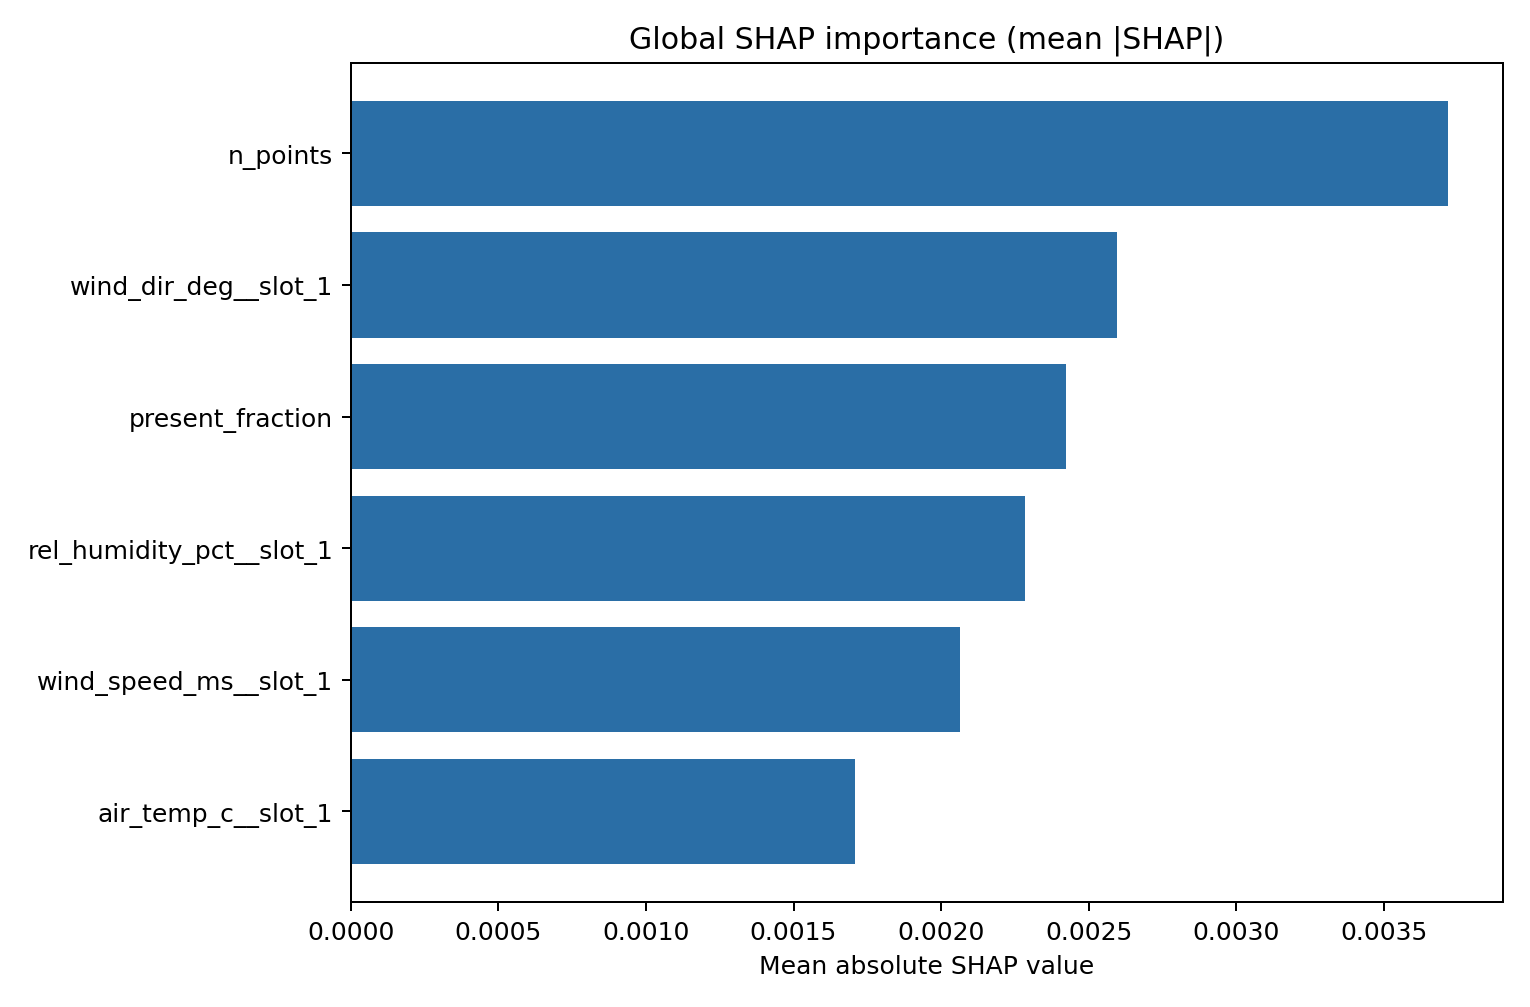
\includegraphics[width=0.98\linewidth]{figures/fig_shap_global_top.png}\\[-2pt]
  {\scriptsize\color{cmuted}Global SHAP: top drivers.}
\end{columns}
\end{frame}

% ── SLIDE 6 ──────────────────────────────────────────────────────────────────
\begin{frame}{Explanation outputs (local + cluster-level)}
\begin{columns}[T,onlytextwidth]
  \column{0.5\textwidth}
  \centering
  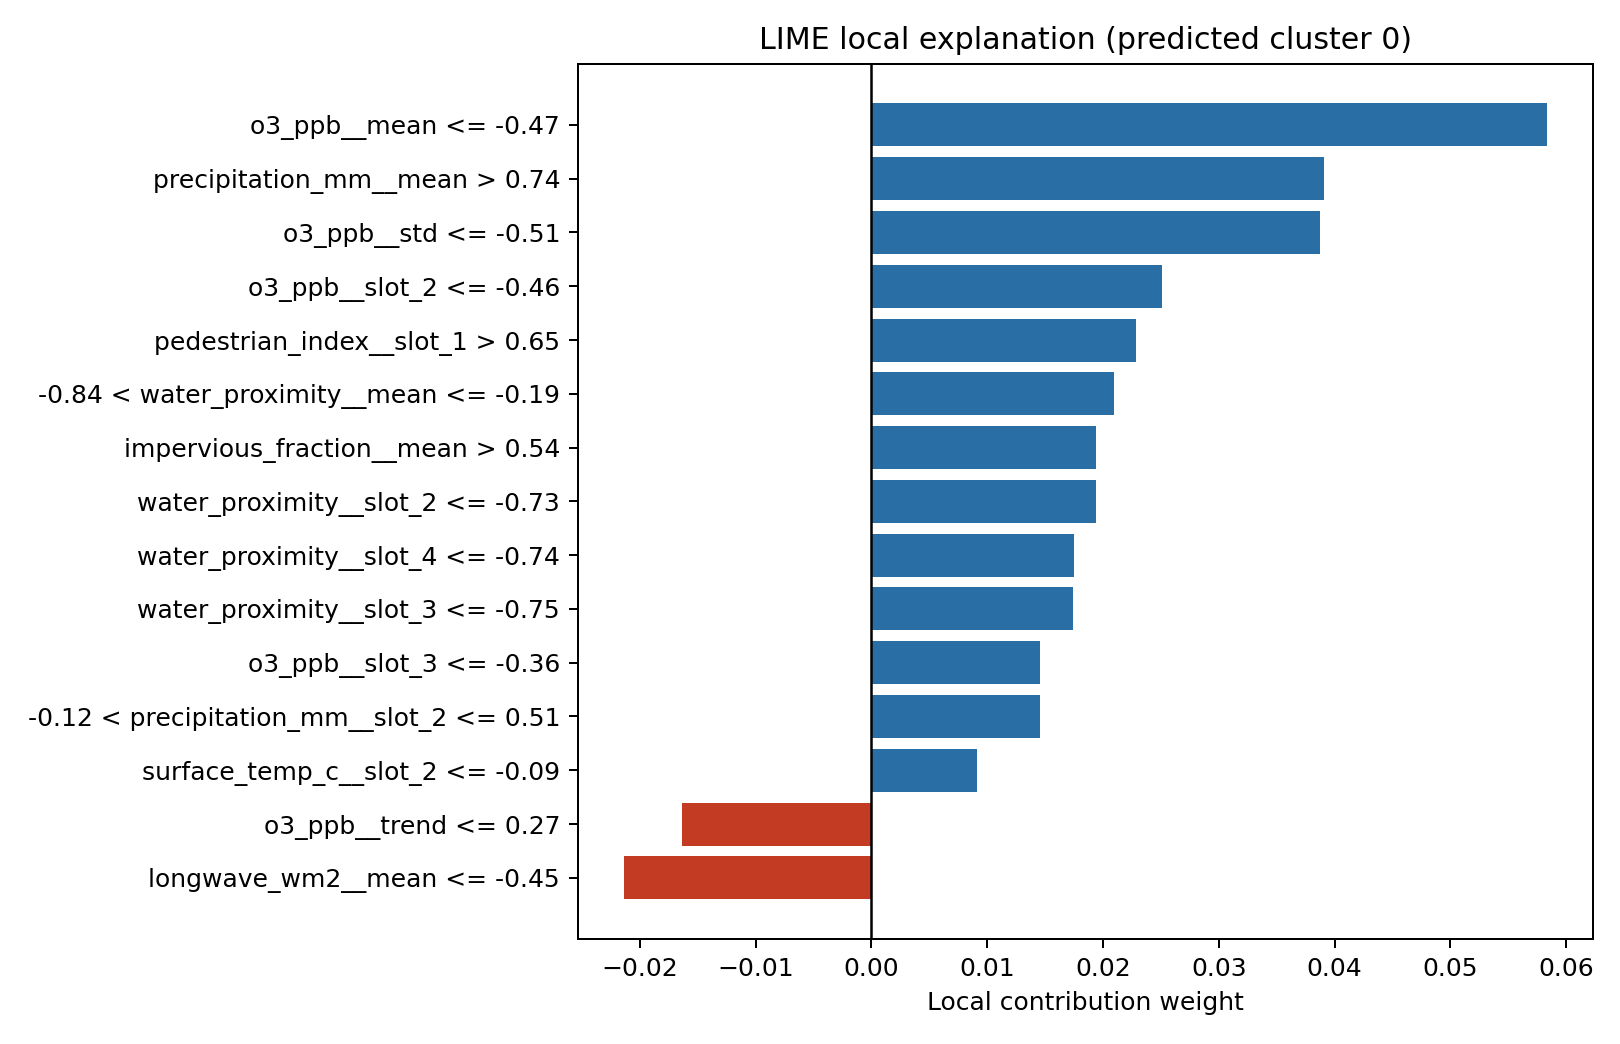
\includegraphics[width=0.98\linewidth]{figures/fig_lime_local.png}\\[-2pt]
  {\scriptsize\color{cmuted}Local LIME explanation (example point).}
  \column{0.5\textwidth}
  \centering
  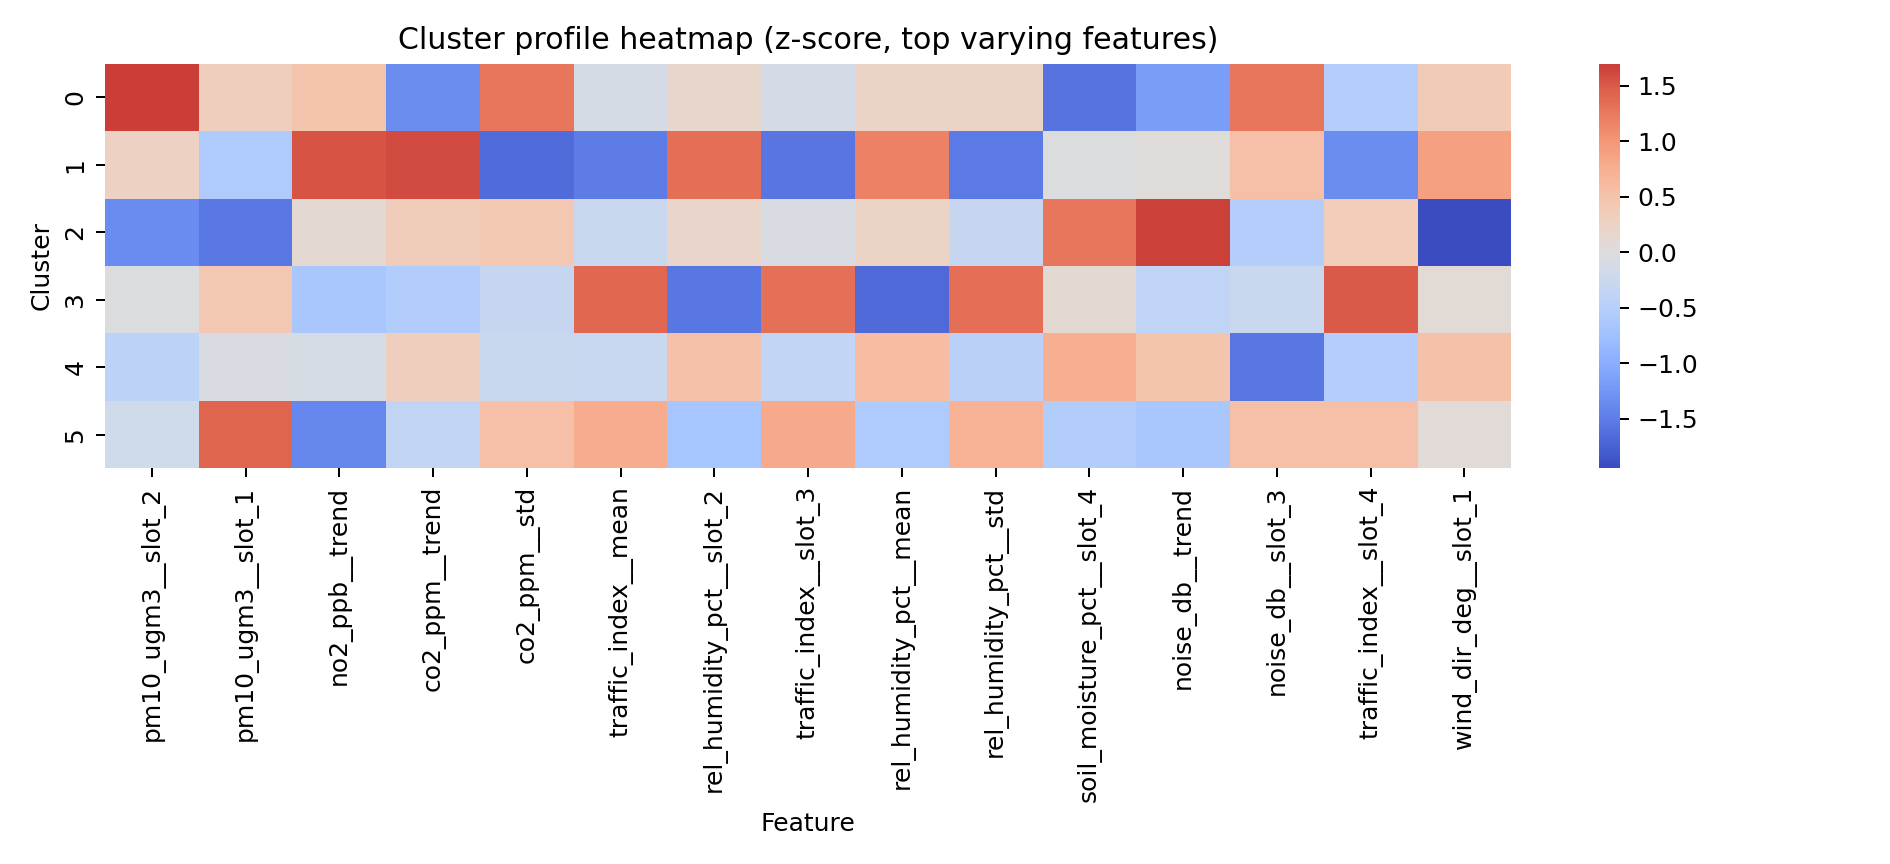
\includegraphics[width=0.98\linewidth]{figures/fig_cluster_driver_heatmap.png}\\[-2pt]
  {\scriptsize\color{cmuted}Cluster driver heatmap (surrogate-based).}
\end{columns}
\end{frame}

% ── SLIDE 7 ──────────────────────────────────────────────────────────────────
\begin{frame}{Surrogate quality + deep baseline}
\begin{columns}[T,onlytextwidth]
  \column{0.5\textwidth}
  \centering
  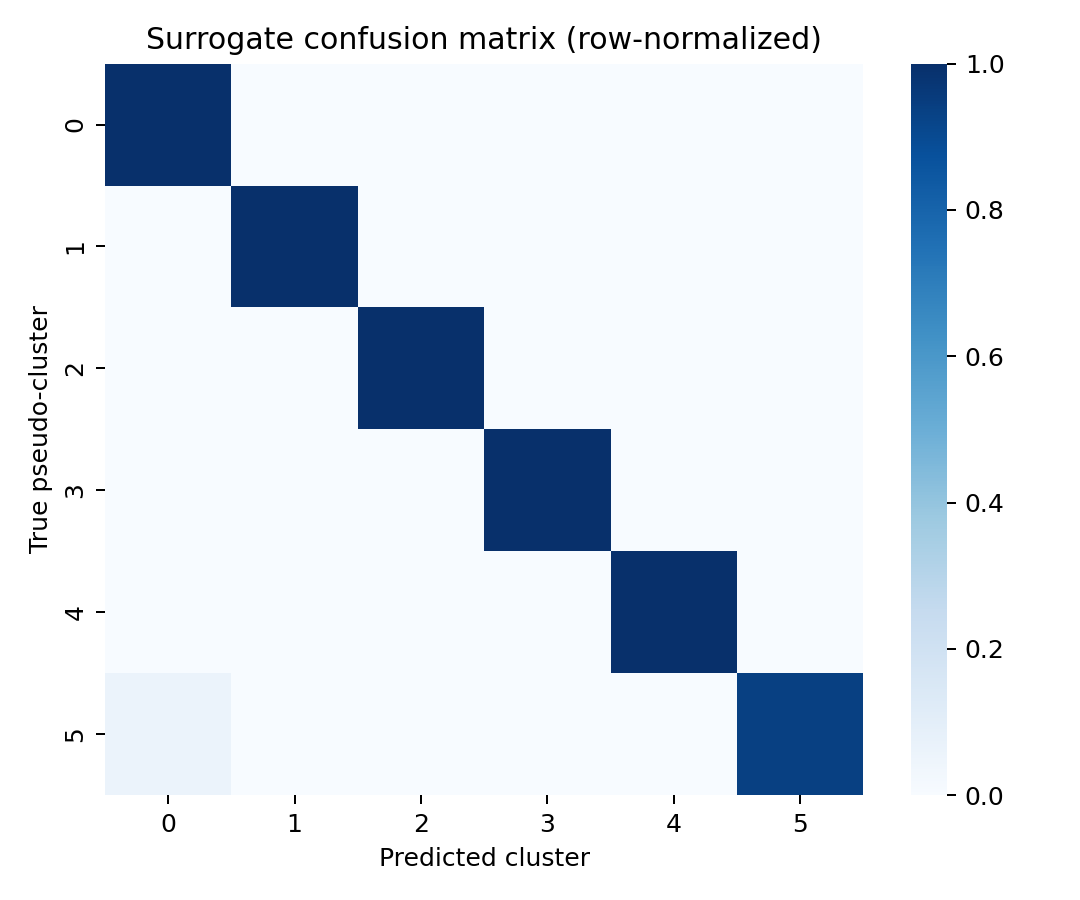
\includegraphics[width=0.98\linewidth]{figures/fig_surrogate_confusion_matrix.png}\\[-2pt]
  {\scriptsize\color{cmuted}Surrogate confusion matrix.}
  \column{0.5\textwidth}
  \centering
  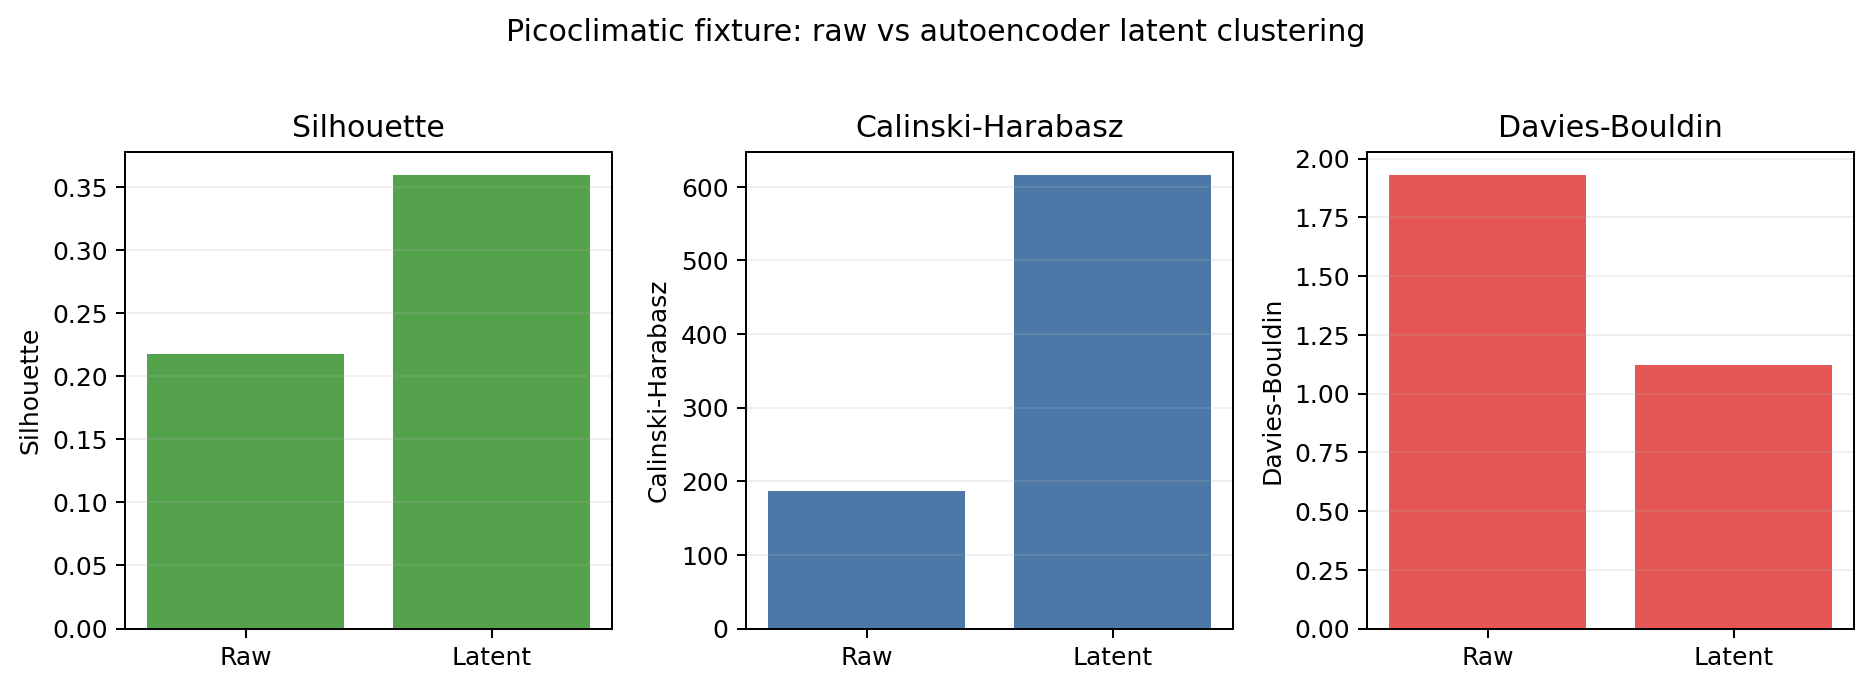
\includegraphics[width=0.98\linewidth]{figures/deep_representation_comparison.png}\\[-2pt]
  {\scriptsize\color{cmuted}Deep representation comparator.}
\end{columns}
\end{frame}

% ── SLIDE 8 ──────────────────────────────────────────────────────────────────
\begin{frame}{Benchmarks + next}
\begin{columns}[T,onlytextwidth]
  \column{0.62\textwidth}
  \centering
  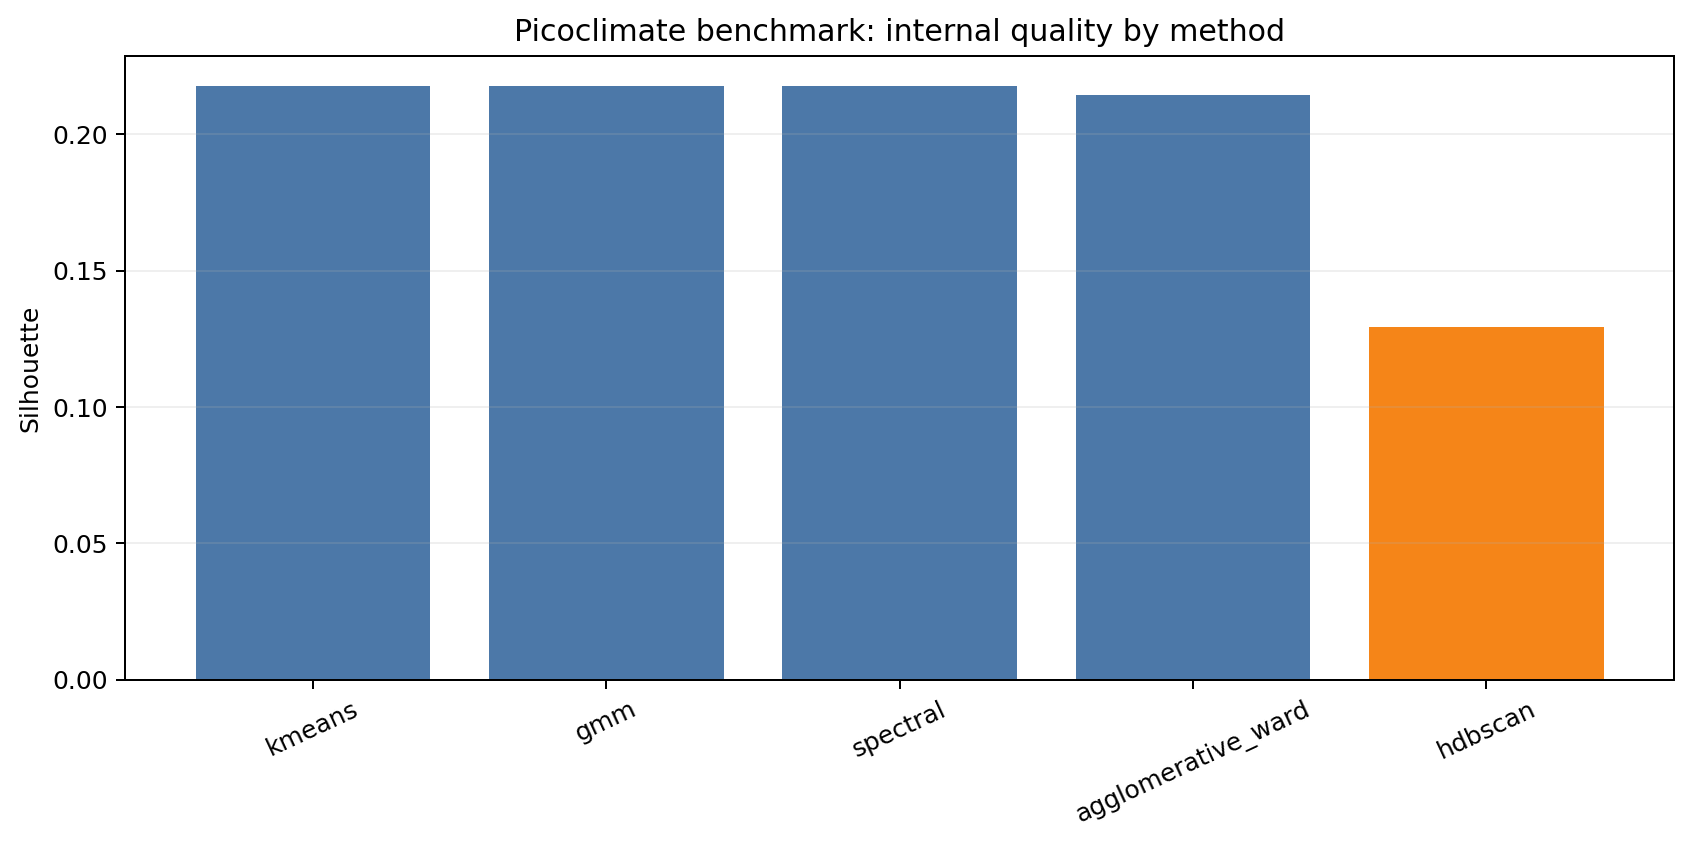
\includegraphics[width=0.98\linewidth]{figures/benchmark_silhouette.png}
  \column{0.36\textwidth}
  \begin{block}{Next}
    \begin{itemize}\footnotesize\setlength\itemsep{3pt}
      \item Freeze explanation schema (sensor-unit language).
      \item Expand benchmark matrix (spatial + deep baselines).
      \item Integrate real PICOPATT data when available.
    \end{itemize}
  \end{block}
\end{columns}
\end{frame}

\end{document}
